\documentclass[11pt, a4paper]{article}
%\DeclareUnicodeCharacter{200A}{!!!FIX ME!!!}

\usepackage[utf8]{inputenc}
\usepackage[margin=1in]{geometry}
\usepackage{txfonts}
\usepackage{blindtext}
\usepackage{listings}
\usepackage{hyperref}
\usepackage{graphicx}
\usepackage{xcolor}
\usepackage{cleveref}

\newsavebox{\mybox}
\savebox{\mybox}[0.5\textwidth][c]{aaaa}
%\renewcommand{\lstlisting}{code}
\renewcommand{\lstlistlistingname}{List of codes}
\lstdefinestyle{chstyle}{%
backgroundcolor=\color{gray!12},
basicstyle=\ttfamily\small,
commentstyle=\color{green!60!black},
keywordstyle=\color{magenta},
stringstyle=\color{blue!50!red},
showstringspaces=false,
captionpos = b,
numbers = left,
numberstyle=\footnotesize\color{gray},
numbersep=10pt,
stepnumber=2,
tabsize = 3,
frame=L,
framerule=1pt,
rulecolor=\color{red},
breaklines = true,}


\title{C++ Tutorials for Beginners}
\author{Kouassi Franck Armand Prince
\date{09.05.2021}
}


\begin{document}

\maketitle\hrule
% \begin{center}
% \textbf{C++ Tutorials for Beginners}
% \end{center}
\newpage

\tableofcontents
\listoffigures
\lstlistoflistings
\pagebreak

\section{Getting Started}
%{\blindtext}
This section introduces the basics of C++ programming language and the tools
needed to follow this tutorial. The goal of this tutorial is to help beginners
getting started with C++ programming language. It does not require you to you to
have a prior programming background kownledge. All you have to do is to follow along
with me and and try to \textbf{\textit{WRITE}} the code on your own machine not just read.
Believe me it is easier to read and assume that you have mastered it until you are required
to write the code by yourself, that is where it realize you have not properly understood it.

\subsection{Understand the Computer Language}
%{\blindtext}
Your computer is an incredible and complicated device. Basically, the computer
understands one simple language composed of 0 and 1. Thus a message like this
"\textit{01001100101001010}" could mean "open a window" for instance. Fortunately, we do not have
to learn this language (Binary language). Programmers created languages which are much simpler
than binary language. Here you could check \href{https://en.wikipedia.org/wiki/List_of_programming_languages}
{\emph{\textit{the number of programming languages.}}} \newline
All programming languages have the same goal, that is being able to easily and efficently
communicate with the computer compare to binary language.\newline Here, is how it works :

1. You write the instructions to be executed by the computer in a programming language (e.g C++)

2. The instructions are translated in binary (0 and 1), the language understood by the computer.

3. The computer can now decode the message and executes your request.

\begin{figure}[!ht]
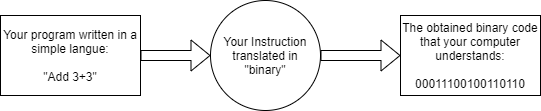
\includegraphics[width = \linewidth]{diagrams/compling.png}
\caption{Compliling Process.}
\label{fig:Compliling Process}
\end{figure}

\subsection{C++ against other programming languages}
Before we start talking about why C++ reprsents a powerful language despite its age. let's discuss the
the key points to analyze before diving into a language.

There exists numerous programming languages as mentioned in above section, although some languages are interesting, 
they are seldom used. The main challenge that comes with these languges, is that they do not have a very big community 
so imagine you working on a project and you are facing a problem, it is difficult to find help since not so many people 
are using the the language.This explains why C++ represents a good choice for debutant programmers. You are not alone, a lot
ressources are availble to guide through your learning process, also C++ is still being widely used.

Another interesting aspect to look at as well is the programming language level. There are of two (02)
types: \textbf{\textit{{high level}}} and \textbf{\textit{{low level}}}.
\newline
\textbf{\textit{{high level}}}: is a language that is that is far from binary language and really
to humans languge,it allows to easily understand and translate instructions contrary to \textbf{\textit{{low level}}}
which a language closed to machine language and generally requires much more effort but gives you more 
control over what you can do, it is a trade-off.

\begin{figure}[h!]
    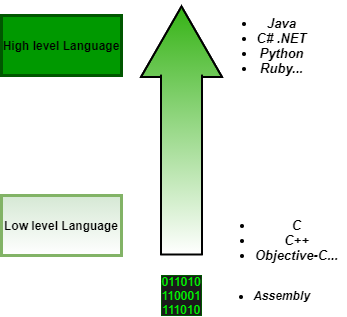
\includegraphics[width = \linewidth]{diagrams/low vs high.png}
    \caption{Programming Language by level.}
    \label{fig:Programming Language by level}
\end{figure}
C++ is a low level language. Do not panic, although coding in C++ might be a little complex, you will 
have in your possession a very \textbf{\textit{{powerful}}} and particulary \textbf{\textit{{fast}}} language.
Infact, if most games are developed in C++, it is because it is the language capable of coupling
speed and power, that makes it an essential language.



\subsection{Summary of C++}
Here we are going to showcase some aspects of C++ that make it an important language regardless of
how long it has been since it creation.
\begin{itemize}
    \item \textbf{Popularity} : C++ is one of the most popular
    languages in the world. It is used by some 4.4 million developers worldwide
    \item \textbf{Large Community} : There is a large online community
    of C++ users and experts that is particularly helpful in case any support is required.
    There is a lot of resources available on the internet regarding C++.
    \item \textbf{Portable} : Programs developed in C++ can be moved from one platform
    to another. This is one of the main reasons that applications requiring multi-platform
    or multi-device development often use C++.
    \item  \textbf{Speed} : Programs written in C++ language execute more faster compare
    to most programming languages\end{itemize}

\paragraph{Snippet of C++}
To give you an idea of how the code looks, let's look at a simple C++ program displaying "Hello world!"
on the screen. Do not try to understand the code just appreciate the beauty and structure. We will
go into details in the following sections

\begin{lstlisting}[caption=Sample example of C++ programming language, style=chstyle,
    language=C++, label = c-sample]
//=================================================
// Sample example of C++ programming language
//=================================================

#include <iostream>

using namespace std;

int main()
{
    cout << "Hello world!" << endl;
    return 0;
}
//=================================================
\end{lstlisting}
\textit{ If you are interested in knowing the story of C++ starting from its creation,
\href{https://en.wikipedia.org/wiki/Bjarne_Stroustrup}{you can learn all about C++ from wikipedia}}

\subsection{Summary}
% \subparagraph{sub paragraph}
% {\blindtext}
\begin{itemize}
    \item Programs allow us to efficently control actions on the computer: web browsing, text editing etc
    \item In order to create a program, we write instructions for the computer using a programming; source code
    \item The source code must be converted in binary by what we could a compiler, it allows the executation 
    of the code.
    \item  C++ is a widely used programming language, it is an evolution of C programming due to the fact that 
    it allows Object Oriented Programming (OOP), a very powerful programming feature.
\end{itemize}
\newpage

\section{Environment setup}
In this section, we are going to introduce the tools needed to follow
this tutorial.From our previous discuss, you already know by now an important
tool needed, Yes you are right, you need a Compiler, the program that
converts your C++ code into the computer readable format.

Aside these, there are additional tools needed for you to code with ease
\begin{itemize}
    \item \textbf{A text editor}: It will allow you to write your source
    code. On windows we have Notepad or Vi on linux. But of course, it is
    less recommed because as your code gets bigger and bigger, you might not 
    not be  able to fully control it.
    \item \textbf{A compiler}: as mentioned above, it converts your source code into
    binary format for the computer
    \item \textbf{A debugger}: it helps you find bugs in your programs.
\end{itemize}
From now on we have two options (02) either we get the programs seperatly
which is of course much complicated, but on Linux most programmers prefer
to use them in that way, I will not go into much details here, instead we
are going to explore the simple way. We can get a program "3 in 1",
Yes you heard me correctly, a tool capable of handling the 3 listed tools
It is commonly refered to as an \textbf{IDE} (Integrated Developement Environment).
There are of numerous types. In this tutorial we are not going to discuss
their similarities. I personnaly recommed Visual Studio Code and here is
how you can \href{https://code.visualstudio.com/docs/languages/cpp}
{get started with C++ for Visual Studio Code}. So go ahead and install the
necessary packages.

\section{Your first C++ code}
The “Hello World” program is the first but most vital step towards
learning any programming language and it is certainly the simplest
program you will learn with each programming language. All you need
to do is display the message "Hello World" on the output screen.
\lstinputlisting[language=c++, style=chstyle, label=first C++ code, caption=First C++ code]{codes/first.c++}

\noindent \textbf{Output:}
\lstinputlisting[style=chstyle, label= hello world, caption=First C++ code Output]{codes/1.txt}

\noindent
\textbf{1}. \fbox{\color{green!60!black}// Your first C++ program }\\
In C++, any line starting with \fbox{\color{green!60!black}//} is a comment. Comments are
intended for the person reading the code to better understand the
functionality of the program. It is completely ignored by the C++
compiler.

\noindent
\textbf{2}. \fbox{\color{magenta}\#include \color{black}\textless iostream\textgreater}\\
The \#include is a preprocessor directive used to include files in our
program. The above code is including the contents of the iostream file.

\noindent
\textbf{3}. \fbox{\color{magenta}int \color{black}main() \{...\}}\\
A valid C++ program must have the main() function. The curly braces
indicate the start and the end of the function. \\ The execution of
code beings from this function.

\noindent
\textbf{4}. \fbox{std::cout \textless\textless \color{blue!50!red}"Hello World!";}\\
std::cout prints the content inside the quotation marks.
It must be followed by '\textless\textless'  followed by the format string.
In our example, "Hello World!" is the format string. \\
\textbf{Note: } \fbox{;} is used to indicate the end of a statement.

\noindent
\textbf{5}. \fbox{\color{magenta}return \color{black} 0;}\\
The return 0; statement is the "Exit status" of the program.
In simple terms, the program ends with this statement.

As you might have noticed, the code in \ref{c-sample} looks a little different from the one
in \ref{first C++ code} but produce the same output do not worry we are going to get to the
difference soon. \\
\noindent In \ref{c-sample}, line 7 we used \fbox{\color{purple!85}using namespace \color{black} std;}
to tell the compiler to use standard namespace. Namespace collects identifiers used for class, object
and variables. Name space can be used by two ways in a program, either by the use of using statement
at the beginning, like we did in above mentioned program or by using name of namespace as prefix
before the identifier with scope resolution (::) operator. Thus with namespace std,
\fbox{std::cout \color{black}\textless\textless \color{blue!50!red}"Hello World!";}
becomes \fbox{cout \textless\textless \color{blue!50!red}"Hello World!";}
like in our previous example, much simpler right !! it is totally up to you, to define on which style
suits you the most.\\
\noindent  also, the keyword \fbox{endl} is used to denote the end of a line therefore, the next line 
of code will be printed on a new line.\\
It is also important to notice that you could combine instructions into a single one. for example,
\lstinputlisting[style=chstyle, language=C++, label=Compress C++ code, caption= Compress C++ code ]
{codes/oneLine.c++}
This code output the two (02) instructions on 02 lines, you can run the code and see the output.

\subsection{Make your code more readable}
In order to allow others and yoursel to understand your code, it is recommended to add
comments to your code. Now we are going to learn how to comment our program. We introduced
the concept of the in the previous section but lets dive depper into it.\\
There exists two (02) types of comments :
\begin{itemize}
\item {\textbf{Short comments}}: as stated in the names they are short and can be written
    in one line of code. To write a short comment, you just need to start with \fbox{\color{green!60!black}//}
    following by your comment.
\end{itemize}
\lstinputlisting[style=chstyle, language=C++, label= First short commment, caption= First short commment]
{codes/comment1.txt}


\begin{itemize}
\item {\textbf{Long comments}}: if your comments are long enough and can not fit in one line,
    you can have a block comment. You just need to start and end your block comment
    with \fbox{/*}.
\end{itemize}

\lstinputlisting[style=chstyle, language=C++, label= First block commment,
caption= First short commment]{codes/comment2.txt}

\noindent Generally, we do not write too much in the comment section, just the necessary
information, unless you have to.

\begin{itemize}
    \item {\textbf{Let's comment our code}}
\end{itemize}
\lstinputlisting[
    style=chstyle, language=C++, label= Comments in C++,
    caption= Comments in C++
]{codes/helloworldCommented.c++}

\noindent After you run this code, nothing will change, the output will still be the same
because comments are simply ignored by the compiler.

\subsection{Summary}
\begin{itemize}
    \item The execution of code begins from the main() function. This function is mandatory.
    This is a valid C++ program that does nothing.
    \item The \fbox{cout} is used to display a message.
    \item You can comment your codes in two (02) ways
    \fbox{// Comment} or \fbox{/* Comment */}
\end{itemize}

\section{Introduction to variables in C++}
So far, you have discovered how to create and compile your first programs in console mode.
Right now these programs are very simple. They display messages on the screen...and nothing
more. This is mainly due to the fact that your programs do not know how to interact
with their users. This is what we will learn to do in the next chapter. But before that we need
to introduce an important concept: \textbf{variables}

\subsection{what is a variable ?}
The one and only thing you need to know is that a variable is a part of the memory that the computer
lends us to put values into it. Imagine that the computer has in its entrails a large wardrobe that
has thousands (billions!) of small drawers; these are places that we will be able to
use to put our variables into.\\
In the case of a simple calculator, one can usually store only one number at a time. As you can
imagine, in the case of a program, we will have to keep more than one thing at the same time.
So you need a way to differentiate the variables to be able to access them afterwards.
So each variable has a \textbf{name}. It is in other words the label that is stuck on the drawer.
\\The other thing that distinguishes the calculator from the computer is that we would like to
be able to store a lot of different things, numbers, letters, sentences, pictures, etc.
This is what we call the type of a variable. You can imagine that as the shape of the drawer.
We do not use the same drawers to store bottles or books.

\subsection{Variables Naming conventions}
Let’s start with the question of variable names. In C++, there are a few rules that
govern the different names allowed or prohibited.
\begin{itemize}
\item Variable names are made up of letters, numbers and the underscore only;
\item The first character must be a letter (upper or lower case);
\item Spaces in the name is not allowed;
\end{itemize}
Here are few examples of valid variables: ageZero, first\_name also, AGEZERO are
allowed variable names. \_ageZero in the other hand is not allowed.\\
To this is added an additional rule, valid for everything written in C++ and not
only for variables. Language makes the difference between upper and lower case.
In technical terms, it is said that C++ is case sensitive. Thus, myAge, myage, MYAGE and
MyAge are all different variables.\\

Personally, I use a \textless\textless convention \textgreater\textgreater shared by many programmers.
In all the big projects with thousands of programmers, there are very strict rules and sometimes difficult
to follow. The ones I propose to you here allow to keep a good legibility and above
all, they will allow you to understand all the examples in the rest of this course.
\begin{itemize}
\item Variable names start with a lower case;
\item If the name is composed of several words, they are put together without space;
\item Each new word (except the first) begins with a capital letter.
\end{itemize}

Let us look at this with examples. Let us take the case of a variable that is supposed
to contain the age of the user of the program.

\begin{itemize}
    \item \fbox{UserAge}: no, because the first letter is a capital letter;
    \item \fbox{user\_age}: no, because the words are not seperated;
    \item \fbox{ageuser}: no, because the second word does not start with a capital letter;
    \item \fbox{ageUser}: ok
\end{itemize}

I strongly advise you to adopt the same convention. Making your code readable and easily
understandable by other programmers is very important, and it doesn’t just involve formatting.

\subsection{Variables types (Data types)}
We learned that a variable has a name and a type. We know how to name our variables, now let’s
see their different types. The computer likes to know what it has in its memory, so you have
to indicate what type of element will contain the variable we would like to use. Is it a number,
a word, a letter? It must be specified.\\

\begin{tabular}{ |p{3cm}||p{10cm}| }
    \hline
    \textbf{Data type} & \textbf{What it contains} \\
    \hline
    bool  & data type with two possible values: true or false    \\
    char&   data type that holds one character (letter, number, etc.) of data  \\
    int &numeric variables holding whole numbers \\
    unsigned int    &A positive or zero integer number.\\
    double&   numeric variables holding numbers with decimal points  \\
    string& data values that are made up of ordered sequences of characters\\
    \hline
\end{tabular}

\subsection{Syntaxt of variable declaration}
In order to declare a variable in C++, the following syntaxt should be applied:
\lstinputlisting[style=chstyle, language=C++, label=Variables Syntaxt,
caption=Variables Syntaxt]{codes/var.txt}
As an example, we have:
\lstinputlisting[style=chstyle, language=C++, label=Variables declaration,
caption=Variables declaration]{codes/var.c++}

\subsubsection{Dealing with strings}
When dealing with strings, the first thing to do is to add a small line at the beginning of your program.
The compiler needs to be told that we want to use strings. Without this, it
would not include the tools needed to manage them. Below is an example:
\lstinputlisting[style=chstyle, language=C++, label=String declaration,
caption=String declaration]{codes/string.c++}

\subsubsection{Dealing with multiple variables}
If you have multiple variables of the same type to declare, you can do so on a single line
by separating them with a comma (,), just like this:
\lstinputlisting[style=chstyle, language=C++, label=Single line declaration,
caption=single line declaration]{codes/multipleVar.c++}

\subsection{Print message on the screen}
As we discussed earlier, the key to print a value on the screen. Now let's combine that to
what we just learn in order to print the value held by our variables. As a remember, the key
was \fbox{cout}. let consider this example:
\lstinputlisting[style=chstyle, language=C++, label=Print message on the screen,
caption=Print message on the screen]{codes/printmsg.c++}
\textbf{Output}
\lstinputlisting[style=chstyle, language=C++, label=message output,
caption=message output]{codes/printMsgOut.txt}

\subsection{Scope of Variables}
All the variables have their area of functioning, and out of that boundary they don't
hold their value, this boundary is called scope of the variable. For most of the
cases its between the curly braces,in which variable is declared that a variable
exists, not outside it. We will study the storage classes later, but as of now,
we can broadly divide variables into two main types:\\
$\bullet$ Global Variables\\
$\bullet$ Local variables

\subsubsection{Global variables}
Global variables are those, which are once declared and can be used throughout
the lifetime of the program. They must be declared
outside the main() function. If only declared, they can be assigned different
values at different time in program lifetime. But even if they are declared and
initialized at the same time outside the main() function, then also they can be
assigned any value at any point in the program. Here is an exmaple:
\lstinputlisting[style=chstyle, language=C++, label=Global variable,
caption=Global variable]{codes/globalVar.c++}
In this code, the variable x was declared and not initialized (given an initial value)
and was updated twice inside the main() function. You can run the code and see the output

\subsubsection{Local variables}
Local variables are the variables which exist only between the curly braces,
in which its declared. Outside that they are unavailable and leads to compile time error.

\subsection{Summary}
\begin{itemize}
\item A variable is an information stored in the memory.
\item There exists various types of variables : \fbox{bool}, \fbox{char}, \fbox{int} ...
\item The value of a variable can be displayed at any time with : \fbox{cout}
\item There exists two types of variables : Global and Local variables
\end{itemize}

\section{How to handle user input}
In the previous chapter, I explained how to display variables in the console. 
Now let’s see how to do the opposite, which is to ask the user for information
to store it in memory. let's look at an example.
\lstinputlisting[style=chstyle, language=C++, label=Saving a variable in the memory,
caption=Saving a variable in the memory]{codes/cin.c++}
\textbf{Output}
\lstinputlisting[style=chstyle, language=C++, label=Saving a variable in the memory output,
caption=Saving a variable in the memory]{codes/cinOut.txt}
The program displayed "how old are are you ?". So far so good, right ? and on line 8,
the program ask for to store an integer in the memory then, at this moment, the program
ask for user input and updates the variable ageUser initially declared to be holding the
value 0. Finally, the program prints a message along with the user input.\\
When you display the value of a variable, the data comes out of the program,
so you use an arrow going from the variable to \fbox{cout}. When we ask the user
for information, it is the opposite, the value comes from \fbox{cin} and goes into the variable.

\subsubsection{Other variables}
Obviously, what I presented to you also works with other types of variables.
Let’s look at that with a small example.
\lstinputlisting[style=chstyle, language=C++, label=Other variables,
caption=Other variables]{codes/otherVar.c++}
I don’t think I even need to explain it. But I would encourage you to test
it to get a full understanding of what’s going on.

\subsection{Problem with space}
Have you tested the previous code by putting your name and surname?
Let’s see what happens.
\lstinputlisting[style=chstyle, language=C++, label=Problem with space example,
caption=Problem with space example]{codes/otherVarOut.txt}
It’s a space problem. When you press the Enter key, the computer copies what
the user wrote into the memory. But it stops at the first space or return
to the line. When it comes to a number, there is no problem because there is
no space in the numbers.\\
for Strings, a question arises. There may very well be a space in a string.
And so the computer will cut in the wrong place, which is after the first word.
In fact, it should be possible to retrieve the whole line rather than just the first word.
In order to do so, we use the \fbox{getline()} function. Later, we will explain in details
what is a function. So if we modify the the previous code by simply replacing the
\fbox{cin \textgreater\textgreater userName; } by \fbox{getline()}
\lstinputlisting[style=chstyle, language=C++, label=getline example,
caption=getline example]{codes/getLine.c++}
\lstinputlisting[style=chstyle, language=C++, label=getline output,
caption=getline output]{codes/getLineOut.txt}

\subsection{Update a variable}
Let’s start by looking at how to change the content of a variable.
We use the "=" symbol to make a value change. If I have a type \fbox{int} variable whose
content I want to change, I write the name of my variable followed by
the "=" symbol and finally the new value.
\lstinputlisting[style=chstyle, language=C++, label=update variables,
label=update variables]{codes/assignVar.c++}

\subsection{Constants}
I told you how to modify variables. I hope you understood! Because
we’re going to do the opposite. I will show you how to declare non-modifiable variables
(constants).\\
Pensez à une calculatrice, qui aura besoin de la constante $\pi$. This value never changes
$\pi$ will always 3.14.\\
But that’s not all. There are also variables whose value never changes but whose value is
not known in advance. Let’s take the result of an operation in a calculator.
Once the calculation is done, the result does not change. The variable that
contains the result is therefore a constant.\\
So let’s see how to declare such a variable.

\subsubsection{declare a constant}
It’s very simple. You declare a normal variable and add the keyword \fbox{const} between the type
and the name. Also it applies to all variables types.
\lstinputlisting[style=chstyle, language=C++, label=declare a constant,
caption=declare a constant]{codes/const.c++}

\subsection{Operators in C++}
Operators are special type of functions, that takes one or more arguments
and produces a new value. For example : addition (+), substraction (-),
multiplication (*) etc, are all operators. Operators are used to perform
various operations on variables and constants.

\subsubsection{Assignment Operator (=)}
Operates '=' is used for assignment, it takes the right-hand side (called rvalue)
and copy it into the left-hand side (called lvalue). Assignment operator is the
only operator which can be overloaded but cannot be inherited. As an example, we have
\fbox{x = 10;} This statement assigns the integer value 10 to the variable x.\\
\textbf{Note:} The assignment operation always takes place from right to left,
and never the other way around. Another example: \fbox{a = b = c = 10}
It assigns 5 to the all three variables: a, b and c; always from right-to-left.

\subsubsection{Basic Arithmetic Operators (+, -, *, /, \%)}

\begin{tabular}{ |p{3cm}||p{5cm}| }
    \hline
    \textbf{Operator} & \textbf{Description} \\
    \hline
    +  & addition    \\
    ** &   Multiplication  \\
    / & Division \\
    \%    &Modulo\\
    \hline
\end{tabular}\\
\newline\textbf{Note:} Modulo operator returns remainder, for example 20 \% 5 would return 0.
\lstinputlisting[style=chstyle, language=C++, label=Example of Arithmetic Operators,
caption=Example of Arithmetic Operators]{codes/arithmetic.c++}

\subsubsection{Assignment Operators}
Assignments operators in C++ are: =, +=, -=, *=, /=, \%= \\
num2 = num1 would assign value of variable num1 to the variable.\\
num2+=num1 is equal to num2 = num2+num1;\\
num2-=num1 is equal to num2 = num2-num1;\\
num2/=num1 is equal to num2 = num2/num1;\\
num2\%=num1 is equal to num2 = num2\%num1;\\
\newline by applying thisto the previous example we have:
\lstinputlisting[style=chstyle, language=C++, label=Assignment Operators,
label=Assignment Operators]{codes/assignment.c++}

\subsubsection{Auto-increment and Auto-decrement Operators}
Here we are going to talk about the following operators: ++ and --.\\
num++ is equivalent to num=num+1;\\
num–- is equivalent to num=num-1;
\lstinputlisting[style=chstyle, language=C++, label=auto increment/decrement,
caption=auto increment/decrement]{codes/increment.c++}

\subsubsection{Logical Operators}
Logical Operators are used with binary variables. They are mainly used in
conditional statements and loops for evaluating a condition. We have \&\&,$\|$ and !
Given two boolean variables b1 and b2.\\
$\bullet$ b1\&\&b2 will return true if both b1 and b2 are true else it would return false.\\
$\bullet$ b1$\|$b2 will return false if both b1 and b2 are false else it would return true.\\
$\bullet$ !b1 would return the opposite of b1, that means it would be true if b1 is false and
it would return false if b1 is true.
\lstinputlisting[style=chstyle, language=C++, label=Logic operators example,
caption=logic operators example]{codes/logicOp.c++}

\subsubsection{Relational operators}
We have six relational operators in C++: ==, !=, \textgreater, \textless,  \textless =,
\textgreater =.

\begin{tabular}{ |p{3cm}||p{10cm}| }
    \hline
    \textbf{Data type} & \textbf{What it contains} \\
    \hline
    ==  & returns true if both the left side and right side are equal   \\
    != & returns true if left side is not equal to the right side of operator. \\
    \textless &returns true if left side is less than right side.\\
    \textgreater& returns true if left side is greater than right.  \\
    \textgreater = & returns true if left side is greater than or equal to right side.\\
    \textless = & returns true if left side is less than or equal to right side\\
    \hline
\end{tabular}

\subsubsection{Bitwise Operators}
There are six bitwise Operators: $\&$, $\|$,\textless\textless, \textgreater\textgreater,
%Tilde, %^
Bitwise operator performs bit by bit processing.\\
\fbox{num1 = 11; //equal to 00001011} and \fbox{num2 = 22; // equal to 00010110}\\
num1 $\&$ num2 compares corresponding bits of num1 and num2 and generates 1 if both bits
are equal, else it returns 0. In our case it would return: 2 which is 00000010 because
in the binary form of num1 and num2 only second last bits are matching.\\
num1 $\|$ num2 compares corresponding bits of num1 and num2 and generates 1 if either
bit is 1, else it returns 0. In our case it would return 31 which is 00011111.\\
num1 () num2 compares corresponding bits of num1 and num2 and generates 1 if they
are not equal, else it returns 0. In our example it would return 29 which is
equivalent to 00011101.\\
~num1 is a complement operator that just changes the bit from 0 to 1 and 1 to 0.
In our example it would return -12 which is signed 8 bit equivalent to 11110100\\
num1 \textgreater\textgreater 2 is left shift operator that moves the bits to the left,
discards the farleft bit, and assigns the rightmost bit a value of 0. In our case output is 44 which
is equivalent to 00101100.\\

\textbf{Note:} In the example below we are providing 2 at the right side of this shift operator
that is the reason bits are moving two places to the left side. We can change this
number and bits would be moved by the number of bits specified on the right side
of the operator. Same applies to the right side operator.\\
num1 \textgreater\textgreater 2 is right shift operator that moves the bits to the right, discards
the far right bit, and assigns the leftmost bit a value of 0. In our case
output is 2 which is equivalent to 00000010
\lstinputlisting[style=chstyle, language=C++, label=Bitwise operator example,
caption=Bitwise operator example]{codes/bitwise.c++}

\subsubsection{Ternary Operator}
This operator evaluates a boolean expression and assign the value based on the result.\\
here is the syntaxt
\fbox{variable num1 = (expression) ? value if true : value if false}.\\
If the expression results true then the first value before the colon (:)
is assigned to the variable num1 else the second value is assigned to the num1.
\lstinputlisting[style=chstyle, language=C++, label=Ternary operator example,
caption=Ternary operator example]{codes/ternary.c++}

\subsection{Summary}
\begin{itemize}
    \item To ask the user to enter information, we use the 
\end{itemize}



\end{document}